\documentclass[dvipdfmx]{article}

\usepackage{amsmath}
\usepackage{graphicx}
\usepackage{titlesec}
\usepackage{tikz}
\usepackage{circuitikz}
\usepackage[T1,T2A]{fontenc}
\usepackage[utf8]{inputenc}
\usepackage[english,russian]{babel}

\titleformat{\section}
            {\normalfont\Large\bfseries}
            {}
            {0pt}
            {Урок \thesection\quad}

\begin{document}

\noindent\makebox[\linewidth]{\rule{\paperwidth}{0.4pt}}
\section{(14.09.18)}
\noindent\makebox[\linewidth]{\rule{\paperwidth}{0.4pt}}

\subsection{Комплексные числа}
\paragraph{}

Введём обозначение для комплексного числа:

\begin{equation*}
  e^{i\varphi} := cos\varphi + isin\varphi
\end{equation*}

\paragraph{}

Комплексные числа могут оказаться полезными при решении задач в координатах. Покажем это на следующей задаче:

\paragraph{Задача}

Точки $A$ и $B$ движутся по прямым $a$ и $b$ так, что расстояние между ними постоянно.
Необходимо доказать, что траектория точки $C$ эллипс, если треугольник $ABC$ прямо подобен некоторому треугольнику $PQR$.

\paragraph{Решение}

Для начала решим задачу для перпендикулярных прямых $a$ и $b$. Пусть $O$ --- точка пересечения $a$ и $b$.
Если $C$ является серединой $AB$, то её траектория --- окружность, потому что $OC$ постоянно и равно $\frac{1}{2}AB$ как
медиана прямоугольного треугольника $OAB$.

\paragraph{}

Обозначим середину $AB$ как $M$, $K$ --- основание перпендикуляра к $AB$ из точки $C$, $a$ --- расстояние от $M$ до $K$,
$b$ --- отношение длины $CK$ к $a$.

\paragraph{}
\noindent\makebox[\linewidth][c]{
\begin{minipage}{0.4\linewidth}
  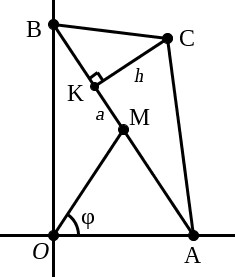
\includegraphics[width=\linewidth,natwidth=235,natheight=277]{images/1.jpg}
\end{minipage}
\begin{minipage}{0.6\linewidth}
  \begin{align*}
    \overrightarrow{OM} &= e^{i\varphi}\\
    \overrightarrow{MK} &= ae^{i(\pi-\varphi)}\\
    \overrightarrow{KC} &= bae^{i(\pi-\varphi)}e^{-i\frac{\pi}{2}}\\
    \overrightarrow{OC} &= \overrightarrow{OM} + \overrightarrow{MK} + \overrightarrow{KC}\\
    \overrightarrow{OC} &= e^{i\varphi} + ae^{i(\pi-\varphi)} + bae^{i(\pi-\varphi)}e^{-i\frac{\pi}{2}}\\
    \overrightarrow{OC} &= e^{i\varphi} - ae^{-i\varphi} + ibae^{-i\varphi}\\
    \overrightarrow{OC} &= \underbrace{e^{i\varphi}}_{z_1} + \underbrace{re^{i\alpha}e^{-i\varphi}}_{z_2},\\
    \text{где } &re^{i\alpha} = -a + iab
  \end{align*}
\end{minipage}}
\paragraph{}



\paragraph{}

\noindent\makebox[\linewidth][c]{
\begin{minipage}{0.4\linewidth}
  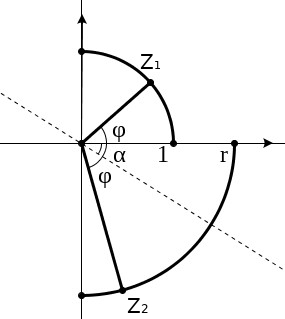
\includegraphics[width=\linewidth,natwidth=285,natheight=319]{images/2.jpg}
\end{minipage}
\begin{minipage}{0.6\linewidth}
  Повернем систему координат так, чтобы ось $OX$ была бисектрисой угла $\alpha$.
  \begin{align*}
    \overrightarrow{OC} &= e^{i\varphi} + re^{-i\varphi}\\
    \overrightarrow{OC} &= cos\varphi + rcos\varphi + i(sin\varphi - rsin\varphi)\\
    \overrightarrow{OC} &= (1+r)cos\varphi + i(1-r)sin\varphi
  \end{align*}
  Замечаем, что мы получили уравнение окружности, сжатой к оси абсцисс в $\frac{1-r}{1+r}$ раз.
\end{minipage}}
\paragraph{}

Решим теперь задачу для неперпендикулярных $a$ и $b$.

\paragraph{}

\noindent\makebox[\linewidth][c]{
\begin{minipage}{0.4\linewidth}
  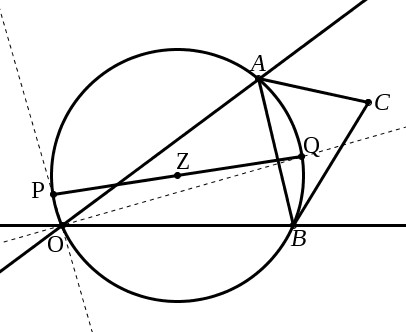
\includegraphics[width=\linewidth,natwidth=406,natheight=332]{images/3.jpg}
\end{minipage}
\begin{minipage}{0.6\linewidth}
  Описанная окружность треугольника $OAB$ имеет постоянный радиус по теореме синусов для угла $\angle AOB$.\\
  Построим радиус $PQ$. $\angle AOQ = 0.5\angle AZQ$ будет постоянным, значит точка $Q$ будет двигаться по прямой $OQ$.
  Аналогично точка $P$ будет двигаться по прямой $OP$.\\
  Замечаем, что $OP \perp OQ$, а значит мы свели задачу к предыдущей.
\end{minipage}}

\end{document}
